\chapter{Damping, Friction, and Energy Dissipation in the Kinematic Chain}
\label{ch:joint_damping_friction}

\section{The Messy Reality of Motion}\label{the-messy-reality-of-motion}

The golfer, club and ball exchange mechanical energy while tissues, interfaces and materials can dissipate some of it. Energy remaining in body motion, elastic storage or gravity is not automatically heat. Muscle metabolic expenditure is also distinct from the mechanical work delivered at the modeled joints. A useful damping model starts with a stated system boundary and an energy ledger.

This chapter separates three questions: where mechanical energy is lost, how a local loss changes coupled motion, and what can be inferred about stability, impact or perceived sweetness. Passive loss does not guarantee better control, worse ball speed or a preferred sound. Those outcomes require a specified trajectory, boundary condition and comparison.

\section{The Hidden Friction in Your
Body}\label{the-hidden-friction-in-your-body}

\subsection{Viscous Damping}\label{viscous-damping}

For a translational coordinate, \(F_d=-cv\) has \(c\) in N s/m. For an angular coordinate, \(\tau_d=-c_\theta\dot q\) has \(c_\theta\) in N m s/rad. The corresponding power is \(-cv^2\) or \(-c_\theta\dot q^2\). The interpretation of a fitted joint coefficient depends on the mechanisms represented by that model; it is not a direct measurement of one tissue's viscosity.

\subsection{Synovial Fluid Viscosity}\label{synovial-fluid-viscosity}

Lubrication and deformation at a joint can contribute resistance, but the phenomenological approximation \(\tau_{\rm fluid}=-c_{\rm fluid}\dot q\) requires identification over a declared posture, loading, temperature and frequency range. It does not establish a constant coefficient for a whole golf swing or a universal monotone dependence on joint size.

\subsection{Muscle Viscosity and the Hill
Model}\label{muscle-viscosity-and-the-hill-model}

An active muscle can deliver positive mechanical work. Its force-velocity relation must therefore not be relabeled as a passive damper. Hill's force-velocity experiment concerns active contraction \citep{Hill1938}; a local slope around a particular activation and operating state is an incremental impedance, not a proof of global passivity. A Hill-type implementation must declare its contraction sign, active and passive elements, moment arms and activation dynamics. A dashpot is a modeling choice, not a mandatory element implied by the historical equation.

For a passive translational dashpot with moment arm \(r\) and local shortening speed \(v=r\dot q\), power consistency gives \(c_\theta=c r^2\). One cannot convert N s/m to N m s/rad without geometry. With multiple muscles, the corresponding Jacobian congruence retains cross-joint coupling.

\subsection{Tendon Viscoelasticity and
Hysteresis}\label{tendon-viscoelasticity-and-hysteresis}

For a closed measured force-extension cycle, the loop integral \(\oint F\,d\ell\) is the mechanical energy not returned over that cycle. A synthetic storage of 10 J with an explicitly assumed 8\% loss would return 9.2 J; this arithmetic supplies no measured tendon percentage or golfer energy budget.

As an illustrative nonlinear loss model, a memoryless quadratic resistance \(-b|\dot q|\dot q\) is passive for \(b\geq0\), but it does not by itself represent viscoelastic memory or identify a measured hysteresis loop across frequencies. Internal-state or hereditary models need their own stored energy, loss law and calibration. Elastic recoil, dissipation and active muscle work remain separate.

\subsection{Ligament Damping and Cartilage
Deformation}\label{ligament-damping-and-cartilage-deformation}

Deformation can store and return energy as well as dissipate it. A model must distinguish these contributions before assigning any residual work to friction. Tissue-specific parameters and injury or clinical conclusions require appropriate identification; this chapter supplies neither a universal joint-loss hierarchy nor an injury-risk model.

\subsection{Soft Tissue Wobble
Damping}\label{soft-tissue-wobble-damping}

Relative soft-tissue motion adds inertial and constitutive states, as discussed in Chapter~\ref{ch:soft_tissue_pliable}. A reduced damping coefficient can approximate a response only in the range over which that reduction is checked. Omitted tissue inertia or resonance must not be concealed by increasing a numerical damping parameter.

\subsection{Damping by Joint}\label{sec-sources_damping}

There is no qualified table of golfer-wide joint damping coefficients in this chapter. The identification requirements are instead:

\begin{center}
\begin{tabularx}{\linewidth}{@{}>{\raggedright\arraybackslash}p{0.27\linewidth}X@{}}
\toprule
\textbf{Modeled Element} & \textbf{Required Coordinates and Evidence} \\
\midrule
Shoulder and scapular motion & Declared relative rotations, posture,
activation and coupled torque response \\
Elbow and wrist & Joint-axis definitions, tendon routing and independent perturbation data \\
Trunk & Distributed or reduced coordinate model and the retained
mechanical boundary \\
Hand-club interface & Colocated force/torque and relative motion, grip
pressure, phase and frequency band \\
Shaft and head & Specimen, boundary conditions, mode shapes, damping and
instrument correction \\
\bottomrule
\end{tabularx}
\end{center}

Passive lower-limb studies are not substitutes for measured shoulder, wrist or grip coefficients. Synthetic sensitivity ranges must be labeled as assumptions and cannot be promoted to physiological uncertainty bounds. \section{Adding Damping to the Equations of Motion} \label{sec:damping_eom}

\index{equations of motion!with damping}

\begin{figure}[htbp]
\centering
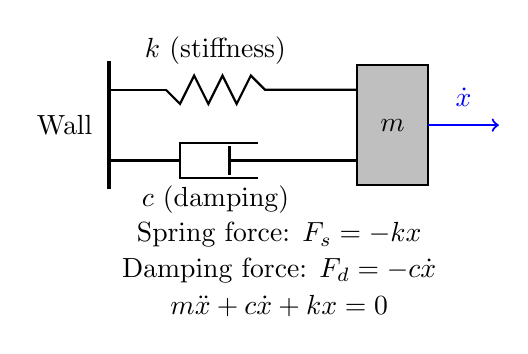
\begin{tikzpicture}[scale=0.9]
  % Both branches join the same fixed wall and translating mass.
  \draw[very thick] (0,-0.9) -- (0,0.9);
  \node[anchor=east] at (-0.1,0) {Wall};
  \draw[thick] (0,0.5) -- (0.8,0.5);
  \draw[thick] (0.8,0.5) -- (1.0,0.3) -- (1.2,0.7)
    -- (1.4,0.3) -- (1.6,0.7) -- (1.8,0.3) -- (2.0,0.7)
    -- (2.2,0.5) -- (3.5,0.5);
  \node at (1.5,1.05) {$k$ (stiffness)};
  \draw[thick] (0,-0.5) -- (1.0,-0.5);
  \draw[thick] (2.1,-0.25) -- (1.0,-0.25) -- (1.0,-0.75) -- (2.1,-0.75);
  \draw[thick] (1.7,-0.7) -- (1.7,-0.3);
  \draw[thick] (1.7,-0.5) -- (3.5,-0.5);
  \node at (1.5,-1.05) {$c$ (damping)};
  \draw[thick,fill=lightgray] (3.5,-0.85) rectangle (4.5,0.85);
  \node at (4,0) {$m$};
  \draw[thick,->,color=blue] (4.5,0) -- (5.5,0);
  \node[color=blue] at (5,0.4) {$\dot{x}$};
  \node at (2.4,-1.55) {Spring force: $F_s=-kx$};
  \node at (2.4,-2.05) {Damping force: $F_d=-c\dot{x}$};
  \node at (2.4,-2.55) {$m\ddot{x}+c\dot{x}+kx=0$};
\end{tikzpicture}
\caption{Parallel Spring and Damper Acting on a Translating Mass. Both Elements Share the Same Displacement and Velocity; Their Forces Add. An Angular Analogue Uses Rotational Inertia and Torques.}
\label{fig:damping_model}
\end{figure}

Recall from Chapter~\ref{ch:parallel_mechanisms} that a kinematic chain with actuator and constraint forces is governed by:
\[
\mathbf{M}(\mathbf{q})\ddot{\bm{q}} + \mathbf{C}(\mathbf{q},\dot{\mathbf{q}})\dot{\bm{q}} + \mathbf{g}(\mathbf{q}) = \bm{B}(\bm{q})\control + \bm{J}_c^T(\bm{q})\boldsymbol{\lambda}
\]

This is a second-order force balance. Its first-order drift field is obtained after defining the state and setting the control input to zero; actuator forces belong to the input term. A phenomenological viscous model adds a separate dissipative force:

\begin{principle}{Damped Kinematic Chain Equations}{damped_eom}
\[
\boxed{\mathbf{M}(\mathbf{q})\ddot{\bm{q}} + \mathbf{C}(\mathbf{q},\dot{\mathbf{q}})\dot{\bm{q}} + \bm{D}(\bm{q})\dot{\bm{q}} + \mathbf{g}(\mathbf{q}) = \bm{B}(\bm{q})\control + \bm{J}_c^T(\bm{q})\boldsymbol{\lambda}}
\]
where the symmetric viscous model used here assumes \(\bm{D}(\bm{q})=\bm{D}(\bm{q})^T\succeq0\). Nonnegative diagonal entries alone do not establish passivity for a coupled matrix. The dissipated power is \(P_d=\dot{\bm q}^{\,T}\bm D\dot{\bm q}\geq0\).
\end{principle}

\index{damping matrix}

The matrix \(\bm D\) maps the declared generalized velocities to generalized dissipative forces. Geometry, activation and internal material states can change an identified response. Neither configuration dependence nor increasing damping with flexion follows merely from choosing the notation \(\bm D(\bm q)\).

\subsection{Types of Damping Models}\label{types-of-damping-models}

Linear viscous damping is useful for a local, frequency-limited approximation. A coupled passive form can be parameterized as \(\bm D=\bm R^T\bm R\); this preserves nonnegative loss without assuming independent joints. Positive diagonal entries alone do not suffice.

Dry sliding friction, rate-dependent drag and viscoelastic memory are different constitutive models. For an angular coordinate, a quadratic torque law uses a coefficient in N m s\(^2\)/rad\(^2\); an aerodynamic translational force coefficient cannot be inserted unchanged. The friction section below states the sliding and sticking conventions explicitly. No universal dominance of linear damping at swing speeds is assumed. \subsection{Rewriting in Control-Affine Form}\label{sec-damping-state-map}

Use local independent joint coordinates with \(\bm v=\dot{\bm q}\) and state \(\mathbf x=(\bm q,\bm v)\). Evaluate the coefficient matrices and gravity force at the current state. For a smooth mode without unresolved constraint forces, \[
\begin{aligned}
\dot{\mathbf x}&=f_0(\mathbf x)+f_d(\mathbf x)+G(\mathbf x)\control,\\
f_0&=\begin{bmatrix}\bm v\\-\bm M^{-1}(\bm C\bm v+\bm g)\end{bmatrix},\\
f_d&=\begin{bmatrix}\bm 0\\-\bm M^{-1}\bm D\bm v\end{bmatrix},\\
G&=\begin{bmatrix}\bm 0\\\bm M^{-1}\bm B\end{bmatrix}.
\end{aligned}
\] Every vector field has \(2n\) components; joint damping forces enter the acceleration block through the inverse mass matrix. A quaternion or other redundant orientation representation instead needs its declared kinematic map \(\dot{\bm q}=\bm N(\bm q)\bm v\). In a closed chain, retain \(\bm J_c^T\boldsymbol{\lambda}\) in the force balance and solve the compatible constraint equations, or eliminate the reactions consistently. The unconstrained \(G\) above cannot simply be reused after that elimination.

\subsection{Conservative Coupling and Dissipated Power}\label{sec-damping-energy-ledger}

The \href{https://underactuated.mit.edu/multibody.html\#the-manipulator-equations}{manipulator-equation derivation in Tedrake's MIT notes} identifies the mass and Coriolis terms together as the contribution of kinetic energy. For a time-independent Lagrangian model with a consistent Coriolis representation, \[
\begin{aligned}
T&=\tfrac12\bm v^T\bm M\bm v,\\
\bm v^T\bm C\bm v&=\tfrac12\bm v^T\dot{\bm M}\bm v.
\end{aligned}
\] One standard choice makes \(\dot{\bm M}-2\bm C\) skew-symmetric; the matrix \(\mathbf{C}(\mathbf{q},\dot{\mathbf{q}})\) itself is not unique. With conservative potential \(V\) and \(\mathbf{g}(\mathbf{q})=\nabla V\), differentiating \(E=T+V\) and substituting the force balance gives \[
\dot E=\bm v^T\bm B\control
+\bm v^T\bm J_c^T\boldsymbol{\lambda}
-\bm v^T\bm D\bm v.
\] The Coriolis contribution cancels the changing kinetic metric; it is not heat loss. Ideal stationary constraints do no work because \(\bm J_c\bm v=0\). Moving constraints can supply or remove energy, so their work must remain in the ledger. Other physical loss laws require their own power terms.

Linearization about a driven trajectory can contain velocity-dependent terms that affect perturbation growth or decay. Those terms are not, by that fact alone, passive viscous damping. For \href{https://affinedrift.com/articles/technology-heavy-hit-impact-coupling.html}{impact and acoustics}, distinguish this inertial redistribution and moving-grip work from identified material/hand losses and acoustic radiation. A quieter or faster-decaying response does not by itself identify which mechanism caused it. \index{control-affine!with damping}

\section{How Damping Propagates Through a Chain}
\label{sec:propagation}

\index{kinematic chain!coupling}

A key observation is that damping at one joint does not affect only that joint. It propagates through the entire chain via the mass matrix coupling, Coriolis coupling, and constraint coupling.

\subsection{Direct Effect: Local Damping}

The most obvious effect is local. Damping at joint $i$ directly opposes angular velocity at that joint:
\[
-D_{ii} \dot{q}_i
\]
This is a force contribution. The resulting acceleration requires the mass and constraint solve; other simultaneous forces can still accelerate the joint.

\subsection{Coupling Through the Mass Matrix}
\label{subsec:mass_coupling}

\index{mass matrix!coupling}

Here is where it gets interesting. Rearranging the damped equation of motion:
\[
\ddot{\bm{q}} = \mathbf{M}(\mathbf{q})^{-1} \left[ \bm{B}\control - \mathbf{C}(\mathbf{q},\dot{\mathbf{q}})\dot{\bm{q}} - \bm{D}\dot{\bm{q}} - \mathbf{g}(\mathbf{q}) \right]
\]

Because $\mathbf{M}(\mathbf{q})$ is \emph{not diagonal}, the terms inside the brackets get "mixed" when inverted. Let's illustrate with a simple two-joint chain: shoulder (joint 1) and elbow (joint 2).

\begin{example}{Shoulder-Elbow Damping Coupling}{shoulder_elbow_coupling}
For a planar two-link illustration with massless links, a point mass $m_1$ at the first link's end and $m_2$ at the second link's end, use absolute first-link angle and relative elbow angle $q_2$. Its exact mass matrix is:
\[
\mathbf{M}(\mathbf{q}) = \begin{pmatrix} m_1 L_1^2 + m_2(L_1^2 + L_2^2 + 2L_1 L_2 \cos q_2) & m_2(L_2^2 + L_1 L_2 \cos q_2) \\ m_2(L_2^2 + L_1 L_2 \cos q_2) & m_2 L_2^2 \end{pmatrix}
\]

The off-diagonal terms $M_{12} = M_{21}$ are nonzero and depend on the elbow angle $q_2$. When we invert this matrix to solve for $\ddot{\bm{q}}$, we get:
\[
\ddot{\bm{q}} = \mathbf{M}(\mathbf{q})^{-1} \cdot (\ldots - \bm{D}\dot{\bm{q}} - \ldots)
\]

Suppose we have damping only at the elbow: $\bm{D} = \text{diag}(0, c_2)$. The damping term entering the inverse is:
\[
-\bm{D}\dot{\bm{q}} = \begin{pmatrix} 0 \\ -c_2 \dot{q}_2 \end{pmatrix}
\]

After multiplication by $\mathbf{M}(\mathbf{q})^{-1}$, the shoulder acceleration $\ddot{q}_1$ receives a contribution from this elbow damping force, even though the shoulder has zero damping directly. Quantitatively:
\[
(\ddot{q}_1)_d = -(\mathbf{M}(\mathbf{q})^{-1})_{12}c_2\dot{q}_2 = \frac{M_{12}}{\det(\mathbf{M}(\mathbf{q}))}c_2\dot{q}_2
\]

This is only the damping contribution to shoulder acceleration. The cross-term \((\mathbf{M}(\mathbf{q})^{-1})_{12}\) couples the two joints; its sign depends on configuration. The determinant already occurs in the inverse and must not be applied a second time. Total passive loss remains \(c_2\dot q_2^2\), even when the shoulder accelerates in the direction of its own motion.
\end{example}

This is crucial: in a multi-joint chain, you cannot treat each joint's dynamics in isolation. The mass matrix creates a network of inertial coupling. Damping at a distal joint propagates proximally.

\subsection{Coupling Through Coriolis Effects}\label{coupling-through-coriolis-effects}

The Coriolis force depends quadratically on the joint velocities at a fixed configuration: \[
\bm C(\bm{q}, \dot{\bm{q}}) \dot{\bm{q}}
\]

Uniformly scaling all velocities by a factor scales this force by the factor squared. Changing one velocity component or the configuration can instead increase, decrease or reverse individual force components. Damping therefore changes subsequent inertial coupling through the trajectory, but it creates no additional Coriolis dissipation beyond the physical loss terms in Section~\ref{sec-damping-energy-ledger}. \subsection{Energy Cascade in Serial Chains}\label{energy-cascade-in-serial-chains}

At a prescribed state with diagonal passive joint damping, the local loss is \(P_i=c_i\dot q_i^2\). The mass matrix affects the resulting accelerations and trajectory, but does not insert an extra downstream inertia multiplier into this instantaneous loss. Neither the proximal nor the distal joint must dissipate more. Relative joint rates must not be replaced by absolute segment rates.

For a synthetic pair with equal \(c_i=0.2\) N m s/rad and rates 10 and 30 rad/s, the losses are 20 and 180 W. Reversing the rates reverses the ranking. Integrating along matched trajectories gives a loss comparison; recomputing a freely evolving swing can also change actuator work and delivered geometry. The previous shoulder/wrist speed estimate and its power ratio are withdrawn because they did not establish those coordinates or measurement conditions.

\subsection{Constraint Coupling in Parallel
Mechanisms}\label{constraint-coupling-in-parallel-mechanisms}

For two hands on different points of a rigid club, hand-point velocities are generally different: a rotating club contributes \(\boldsymbol\omega\times\mathbf r\) at each offset. Express all twists and wrenches in declared compatible frames. Let \(\mathbf q=(\mathbf q_L,\mathbf q_R,\mathbf q_c)\) include both arms and the club, and let the no-slip closure be \(\mathbf J_c\dot{\mathbf q}=0\). Ideal reactions are \(\mathbf J_c^T\boldsymbol\lambda\), with

\[
P_{\rm constraint}=\dot{\mathbf q}^{\,T}\mathbf J_c^T\boldsymbol\lambda=0.
\]

Separate generalized torques of arms with different coordinate spaces cannot simply be added and set to zero. Club force and moment balance retains its inertia, external loads and both contact wrenches. Ideal internal constraints redistribute work between components without creating extra total loss.

If \(\dot{\mathbf q}=\mathbf N\dot{\mathbf s}\) with \(\mathbf J_c\mathbf N=0\), then \(\mathbf D_r=\mathbf N^T\mathbf D\mathbf N\) and \(\dot{\mathbf s}^{\,T}\mathbf D_r\dot{\mathbf s}=\dot{\mathbf q}^{\,T}\mathbf D\dot{\mathbf q}\). This proves preserved nonnegative loss while allowing off-diagonal reduced coupling. A changing basis also contributes kinematic terms to the dynamics. Moving constraints have prescribed nonzero velocity and can perform work; compliant or slipping contacts require explicit port laws rather than ideal no-slip closure.

\section{The Damping Paradox}\label{sec:damping_paradox}\label{the-damping-paradox}

\subsection{Damping and Stability}\label{damping-and-stability}

For an autonomous linear perturbation model,

\[
\mathbf M\ddot{\mathbf x}+(\mathbf G+\mathbf C)\dot{\mathbf x}+\mathbf K\mathbf x=0,
\]

assume constant symmetric positive definite \(\mathbf M,\mathbf K\), skew \(\mathbf G\), and symmetric positive semidefinite \(\mathbf C\). Then \(E=\tfrac12\dot{\mathbf x}^T\mathbf M\dot{\mathbf x}+\tfrac12\mathbf x^T\mathbf K\mathbf x\) is positive definite and \(\dot E=-\dot{\mathbf x}^T\mathbf C\dot{\mathbf x}\leq0\). This proves Lyapunov stability. Asymptotic stability additionally requires that the largest invariant set with zero dissipation contain only the equilibrium. Positive definite \(\mathbf C\) suffices under these assumptions; semidefinite damping can leave undamped modes.

With negative stiffness, even the scalar dimensionless equation
\(\ddot x+\dot x-x=0\) retains the growing rate \((\sqrt5-1)/2\). A
stronger counterexample has \(\mathbf M=\mathbf I\),
\(\mathbf K=-\mathbf I\) and
\(\mathbf G=\begin{bmatrix}0&-3\\3&0\end{bmatrix}\). With
\(\mathbf C=0\) its four distinct rates are \(\pm i(3\pm\sqrt5)/2\).
Adding the passive \(\mathbf C=0.1\mathbf I\) produces a pair with
positive real parts. Energy loss and instability coexist because the
equilibrium energy is indefinite. Dissipation-induced instability is a
documented phenomenon \citep{bloch1994dissipation}, not a claim that
this particular instability occurs in a golf club.

A nonsymmetric loaded tangent, accelerating frame or time-varying swing requires its own stability analysis. Frozen eigenvalues and a nonsingular frequency response do not establish stable time evolution. Physical damping must remain separate from numerical stabilization.

\subsection{Underdamped vs.~Overdamped
Joints}\label{underdamped-vs.-overdamped-joints}

For one constant-coefficient scalar oscillator with positive inertia \(I\), stiffness \(k\) and damping \(c\), define \(\omega_n=\sqrt{k/I}\) and \(\zeta=c/(2\sqrt{kI})\). Values \(0<\zeta<1\), \(\zeta=1\) and \(\zeta>1\) distinguish oscillatory, repeated-real and distinct-real decay rates. At \(c=0\) oscillations do not decay. Critical damping gives the familiar nonoscillatory step response for zero initial conditions; arbitrary initial velocity can still cause a crossing of equilibrium, and no universal optimal energy-dissipation objective follows.

A joint embedded in a coupled active chain need not have a single independently meaningful damping ratio. Identify modes or a matrix impedance over the relevant operating range. The chapter does not infer that all human joints are underdamped or that a wrist swing exploits a particular resonance.

\subsection{Active Damping and
Co-Contraction}\label{active-damping-and-co-contraction}

Impedance control concerns the dynamic relationship between motion and applied wrench \citep{hogan1985impedance}. For a local restoring force on the modeled limb, one convention is \(\mathbf f=-\mathbf K(\mathbf x-\mathbf x_d)-\mathbf C(\dot{\mathbf x}-\dot{\mathbf x}_d)\). The sign reverses for the reaction exerted on its environment. A moving target can perform work even when the relative loss is passive.

Co-contraction can alter an identified impedance, but does not supply a universal independent adjustment of stiffness and damping. The identified change depends on activation, reflex delay, posture and task. Passive tissue loss and work by active control must be retained separately; an assumed change during transition is a hypothesis requiring measurement.

\subsection{The Loose Grip Debate}\label{the-loose-grip-debate}

The relevant question is how the identified hand-club impedance depends on pressure, posture, frequency and amplitude. A grip can change storage, inertia, damping, contact area and slip together. It is not enough to assign one scalar damper or assume that tighter grip always improves control and reduces ball speed.

Chiementin and colleagues studied one participant and one hybrid club. Their modal results generally show increased bending damping with firmer grip, but their conclusion states the opposite trend. Their numerical impact response also contains algorithmic damping that is not independently separated from material loss. Preserve these limitations; this study does not establish a universal optimum grip pressure or broadband impact sound prediction \citep{chiementin2019grip}.

The guitar analogy depends on mode-dependent contact: touching where a mode moves can change its decay, while a node can reduce coupling to that mode. A flexible head and shaft have different modes and radiation efficiencies. A shorter ringdown at the grip is not automatically quieter sound at the listener or a sweeter hit. Compare calibrated sound and hand vibration separately, then use blinded perception experiments.

\section{Friction Models for Joints}\label{sec:friction_models}\label{friction-models-for-joints}

\subsection{Coulomb Friction}\label{coulomb-friction}

For a scalar angular sliding coordinate, use \(\tau_f=-\tau_k\operatorname{sign}(\dot q)\) when \(\dot q\ne0\), with \(\tau_k\geq0\) in N m. At a simple interface, \(\tau_k=\mu_k N r\) requires the effective moment arm \(r\). Distributed contact requires integration of traction and lever arm. The product \(\mu_k N\) alone is a force, not a joint torque.

\subsection{Stiction and Reversal
Points}\label{stiction-and-reversal-points}

At zero slip velocity, static friction is set-valued: \(\tau_f\in[-\tau_s,\tau_s]\). Solve force balance and the sticking constraint together; slip begins when the required reaction exceeds the admissible bound. Setting \(\operatorname{sign}(0)=0\) cannot represent nonzero sticking force. Different joints need not reverse simultaneously, and a swing transition is not evidence that an anatomical joint behaves like a dry bearing.

\subsection{The Stribeck Effect}\label{subsec:stribeck}\label{the-stribeck-effect}

An explicitly phenomenological sliding law is

\[
\begin{aligned}
h(v)&=\tau_k+(\tau_s-\tau_k)e^{-(|v|/v_s)^2},\\
\tau_f(v)&=-h(v)\operatorname{sign}(v)-cv,\qquad v\ne0.
\end{aligned}
\]

Here \(\tau_s\geq\tau_k>0\), \(v_s>0\), and \(c\geq0\). The dry-friction magnitude approaches \(\tau_s\) at vanishing nonzero speed and \(\tau_k\) at high speed; the viscous term can still grow. Power is \(-h(v)|v|-cv^2\leq0\). The separate zero-speed inclusion handles sticking. This fixes the reversed limits in the previous expression and does not identify a golfer's joint law.

\subsection{LuGre Friction Model}\label{lugre-friction-model}

A bristle-state model can represent presliding memory \citep{canudas1995friction}. Under a rotational convention with \(z\) in rad and \(h(v)\) in N m, one possible notation is

\[
\dot z=v-\sigma_0|v|z/h(v),\qquad
\tau_{\rm resistance}=\sigma_0z+\sigma_1\dot z+\sigma_2v.
\]

The torque applied against motion is \(-\tau_{\rm resistance}\). State storage means instantaneous returned power need not be zero: passivity must be checked against a declared storage function and admissible parameters. Define initialization, units, steady sliding and numerical handling before use. This is a model option, not a validated anatomical law; its necessity depends on the measured phenomena and validation target.

With $\sigma_0>0$ in N m/rad and $\sigma_1,\sigma_2\geq0$ in N m s/rad, the candidate storage $S=\tfrac12\sigma_0 z^2$ gives
\[
\tau_{\rm resistance}v-\dot S
=\frac{\sigma_0^2|v|z^2}{h(v)}+\sigma_1\dot z\,v+\sigma_2v^2.
\]
For $\sigma_1=0$ this is nonnegative. With bristle damping, the cross term need not be nonnegative, so coefficient positivity alone does not make this storage a certificate for the full output. For a synthetic instantaneous state with $\sigma_0=\sigma_1=1$, $\sigma_2=0$, $z=0.2$, $v=1$ and $h(v)=0.1$ in the stated units, $\dot z=-1$ and the right-hand side is $-0.6$ W. Check the permitted initial states and constitutive operating range before accepting or rejecting a complete passivity claim.

\subsection{Friction Criticality at the
Transition}\label{friction-criticality-at-the-transition}

At sticking, friction can support a force with zero mechanical power. During sliding, loss depends on slip displacement and traction, not on counting reversals. A smooth-looking or jerky transition alone cannot quantify dissipation. No universal 20 ms transition, simultaneous peak tissue stretch or optimal friction level is inferred here. Measure motion, forces and internal states over a defined interval before assigning a transition loss.

\section{Energy Dissipation Budget}\label{sec:energy_budget}\label{energy-dissipation-budget}

\subsection{Sources of Dissipation}\label{sources-of-dissipation}

For a closed mechanical model with explicitly accounted boundary inputs,

\[
E(t_1)-E(t_0)=W_{\rm actuators}+W_{\rm boundary}-E_{\rm losses}.
\]

Include translational and rotational kinetic energy of every retained component, gravity, strain energy and internal constitutive storage in \(E\). Define the system boundary before allocating aerodynamic, interface and radiated-acoustic energy: a flux leaving one subsystem can be stored in another. Avoid counting the same fitted residual as both tissue damping and grip loss.

\subsection{Interpretation}\label{interpretation}

For a synthetic ledger, \(E(t_0)=20\) J, actuator work 100 J, moving-boundary work 5 J and losses 15 J give \(E(t_1)=110\) J. If clubhead kinetic energy is 40 J, the other 70 J may remain in the modeled body, shaft and potential energy. It is not an additional 70 J dissipation. These numbers are an accounting example, not an amateur-golfer energy budget or a metabolic efficiency estimate.

\section{Implications for Swing
Modeling}\label{implications-for-swing-modeling}

\subsection{When Damping Is
Negligible}\label{when-damping-is-negligible}

Neglect a loss only after a sensitivity or error-budget check for the quantity of interest. A small change in ball speed can coexist with a large change in a narrow resonance or ringdown. A zero instantaneous velocity removes a viscous power term at that instant; it does not establish negligible damping over the surrounding interval or eliminate static forces.

\subsection{When Damping Is Critical}\label{when-damping-is-critical}

The importance of a loss depends on the excited modes, their frequencies and motion at dissipative ports, the duration of contact and the observation window. Separate pre-impact trajectory changes, forces during contact and vibration after separation. Post-separation damping cannot change the launch state already established, although it can change sound and feel.

\subsection{Sensitivity Analysis}\label{sensitivity-analysis}

For a declared scalar damping parameter \(d\) and reproducible comparison protocol,

\[
\Delta v_{\rm club}\approx\frac{\partial v_{\rm club}}{\partial d}\Delta d.
\]

There is no extra minus sign: the derivative already carries its sign. A synthetic derivative of \(-0.02\) m/s per N m s/rad with \(\Delta d=5\) N m s/rad gives \(-0.1\) m/s, approximately \(-0.224\) mph using 1 mph = 0.44704 m/s. This is neither a measured derivative nor a 2 mph effect. State whether controls, delivery state, trajectory or external impulse are held fixed, and check finite-difference step convergence where used. A chosen 50\% parameter sweep is scenario analysis, not a confidence interval.

\subsection{Recommendations for
Modelers}\label{recommendations-for-modelers}

Model choice depends on the requested observable and on reproducing the specified measurements within their uncertainty. Record coordinates, force signs, units, boundary work, source data and the qualified frequency/amplitude range. Distinguish calibration from held-out validation and report null effects.

Separate physical damping from integration damping; refine time step, mesh and retained modes without retuning coefficients to hide numerical error. Test stationary, moving-support, free and clamped limits. Inspect stability and passivity independently of solver convergence. Unknown losses must remain unknown rather than becoming default golfer coefficients.

\section{Damping in the Shaft}\label{sec:shaft_damping}\label{damping-in-the-shaft}

\subsection{Material Damping}\label{material-damping}

A recorded decay can combine shaft material loss, head and adhesive loss, grip/fixture dissipation, radiation and instrumentation. It is not automatically intrinsic material damping. Identify the specimen, layup, mode and boundary condition. A material name or flex rating alone cannot rank full-club decay or ball speed.

\subsection{Quality Factor (Q-Factor)}\label{quality-factor-q-factor}

For a lightly damped isolated mode, \(Q\approx1/(2\zeta)\) relates a conventional quality factor to modal damping ratio. With \(x(t)=A e^{-\zeta\omega_n t}\cos(\omega_d t+\phi)\) and \(\omega_d=\omega_n\sqrt{1-\zeta^2}\), the logarithmic decrement is \(\delta=2\pi\zeta/\sqrt{1-\zeta^2}\). The energy lost between corresponding peaks is a fraction \(1-e^{-2\delta}\). Thus defining \(Q\) directly as \(2\pi\) times starting energy divided by that finite-cycle loss agrees with \(1/(2\zeta)\) only in the weak-loss limit.

For a synthetic 100 Hz mode with \(\zeta=0.01\), the conventional \(Q=50\), the amplitude time constant is about 0.159 s, and the corresponding peak-to-peak energy loss is about 11.8\%. Higher \(Q\) means weaker fractional damping under these conventions; it does not mean higher stiffness. The previously unsourced steel/graphite ranges and contradictory material ranking are withdrawn.

\subsection{Lead-Lag Dynamics and
Damping}\label{lead-lag-dynamics-and-damping}

Before impact, mass, stiffness, pre-existing shaft deformation and velocity, applied wrenches and losses determine the delivered state together. After impact, observed motion depends on which bending, torsional and head modes were excited. A claim that shaft damping is negligible during the downswing needs a qualified calculation or measurement for that model and observable.

\subsection{Practical Implications}\label{practical-implications}

For a frozen small perturbation with point-motion map \(\mathbf L\) and the \(e^{i\omega t}\) convention, the impact-point mobility is

\[
\mathbf Y(\omega)=i\omega\mathbf L
\left[\mathbf K-\omega^2\mathbf M+i\omega(\mathbf G+\mathbf C)\right]^{-1}\mathbf L^T.
\]

The transpose maps point wrench back to generalized force and preserves power. Translational and rotational rows have different units. Replacement of a constant-coefficient boundary by an identified frequency-dependent grip impedance depends on its qualification, but its storage and loss must not be counted twice. At a finite preload, differentiating the configuration-dependent port map also contributes geometric tangent terms. A singular or unresolved pencil requires refusal or a qualified alternative formulation, not an arbitrary pseudoinverse.

\subsection{Material Damping and Shaft
Behavior}\label{material-damping-and-shaft-behavior}

Rotation-induced stress can change the tangent stiffness, while Coriolis terms change dynamic coupling. Tension, centrifugal terms, bending and the grip boundary must be derived from one consistent loaded configuration; they do not universally increase every frequency or create extra dissipative loss. A held pose in a rotating observer does not imply a stationary support in the laboratory.

The implementation program in Tools \#5072 retains these distinctions in its loaded chain and finite grip ports. Its synthetic balance and operator tests establish numerical verification only. Contact duration and offset, flexible-head response, acoustic radiation, microphone transfer and physical validation remain separate steps. A claim that one player's strike is sweeter requires matched-delivery analysis and blinded listening evidence, not a ranking of shaft material names. \section{The Control-Affine Perspective on Damping} \label{sec:damping_control_affine}

\index{control-affine!damping}
\index{drift field!damping}

In the control-affine framework, damping modifies the drift field. Recall:
\[
\dot{\state} = f_0(\state) + G(\state)\control
\]

For the independent-coordinate viscous model in Section~\ref{sec-damping-state-map}, the drift field becomes: \[
f_{\text{damped}}(\mathbf{x}) = f_0(\mathbf{x})
+\begin{bmatrix}\bm 0\\-\mathbf{M}(\mathbf{q})^{-1}\bm D\bm v\end{bmatrix}.
\]

Configuration-dependent passive coefficients may represent identified losses within their calibration range. Coulomb friction, viscoelastic memory and active muscle dynamics need their own constitutive states or force laws; they cannot generally be folded into a constant viscous matrix. Coriolis terms remain in the conservative drift and are excluded from the dissipated-power budget.
\begin{driftcontrol}{Damping as Drift Modification}{drift:damping_modification}
For an unforced system with stationary ideal constraints, passive damping makes total mechanical energy nonincreasing. Gravity and joint coupling can still increase an individual joint's speed, and energy decay alone does not prove stability of every equilibrium or driven trajectory. When a particular trajectory is prescribed, inverse dynamics determines the additional actuator work associated with damping. This bookkeeping does not establish a universal muscular strategy for reversing the swing.
\end{driftcontrol}

\section{Summary: The Damping
Principle}\label{summary-the-damping-principle}

Passive loss, energy redistribution, active work and numerical damping are distinct. Coupling changes which motions and ports are excited, while geometry and operating state change the loaded response. Neither energy decay nor a successful solve establishes stability, a launch advantage or perceived sweetness. Report those quantities with their own assumptions and evidence.

\section{Chapter Exercises}\label{chapter-exercises}

All numerical inputs below are synthetic verification cases, not golfer parameter estimates.

\begin{itemize}
\item \textbf{Damping Coefficient Estimation.} For this synthetic case, use \(c_w=0.1\) N m s/rad and \(\dot q_w=50\) rad/s. Find the resisting torque and instantaneous loss power. Compare the torque magnitude with an assumed available 20 N m; explain why this fraction is not a metabolic efficiency.
\item \textbf{Energy Dissipation in a Two-Joint Chain.} For this synthetic case, use rates 10 and 30 rad/s and coefficients 0.5 and 0.15 N m s/rad. Compute total loss power and its ratio to an assumed 400 W mechanical actuator input. Explain why joint location alone does not determine the ratio.
\item \textbf{Damping Ratio and Step Response.} For this synthetic case, a scalar angular oscillator has inertia \(I=0.05\) kg m\(^2\), stiffness \(k=5\) N m/rad and damping \(c=0.2\) N m s/rad. Compute \(\omega_n\), \(\zeta\) and the approximate 2\% step-response settling estimate \(4/(\zeta\omega_n)\). State its assumptions and distinguish rotational inertia from mass.
\item \textbf{Coulomb vs.~Viscous Friction.} For this synthetic case, an idealized contact has \(\mu_k=0.1\), normal force 50 N and moment arm 0.02 m. Find its sliding torque and the angular speed at which \(c=0.5\) N m s/rad gives equal viscous torque. Explain why zero-speed sticking needs a force-balance inclusion.
\item \textbf{Configuration-Dependent Damping.} For this synthetic case, on the explicitly restricted interval \(0\leq q\leq1\) rad, let \(c(q)=0.1+0.02q\) N m s/rad and \(\dot q=50\) rad/s. Compute torque at \(q=0,0.5,1\). Check nonnegative loss and distinguish this assumed law from measured posture dependence.
\item \textbf{Stability Counterexample.} Calculate the roots of \(\ddot x+\dot x-x=0\) and identify why the positive-stiffness energy argument fails. Repeat for the two-coordinate gyroscopic example with and without \(0.1\mathbf I\) damping.
\item \textbf{Grip and Sound.} Design a comparison that separates changed delivery, changed impact-point mobility, radiated sound and listener preference. State which data would falsify a proposed grip-damping mechanism and which quantities a shaft accelerometer alone cannot identify.
\end{itemize}
